\documentclass[tikz, border=10pt]{standalone}
\usepackage{pgfplots}
\usepackage{amsmath}
\usetikzlibrary{backgrounds}
\pgfplotsset{compat=1.18}

\begin{document}
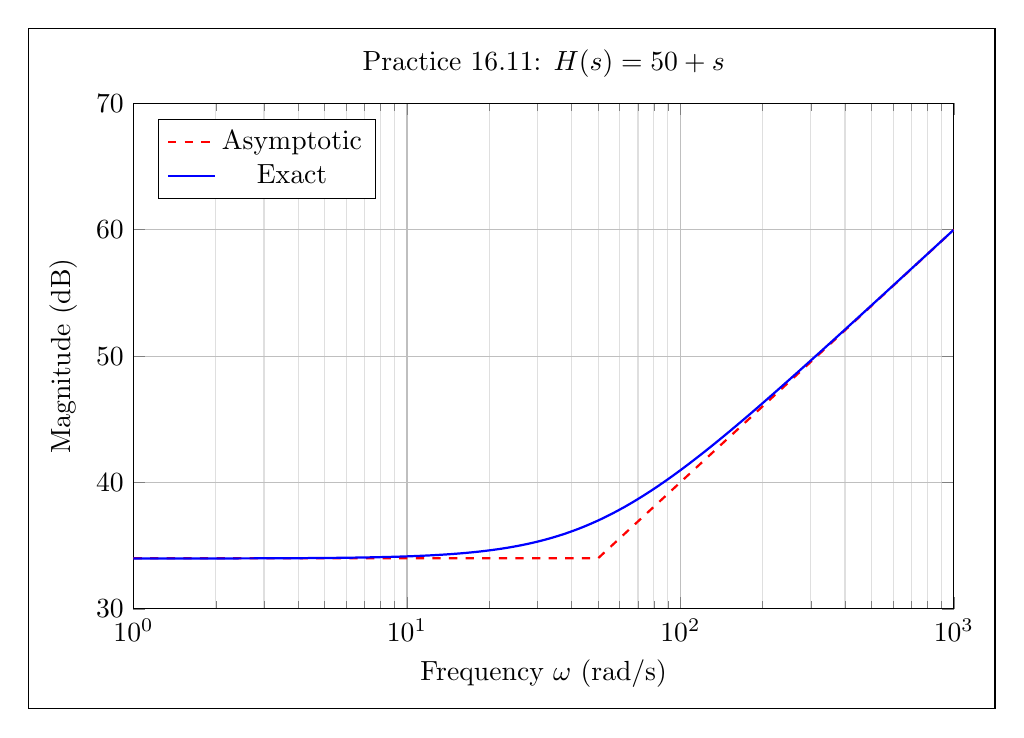
\begin{tikzpicture}[show background rectangle]
    \begin{semilogxaxis}[
        width=12cm, height=8cm,
        title={Practice 16.11: $H(s) = 50 + s$},
        xlabel={Frequency $\omega$ (rad/s)},
        ylabel={Magnitude (dB)},
        grid=both,
        xmin=1, xmax=1000,
        ymin=30, ymax=70,
        minor grid style={gray!25},
        major grid style={gray!50},
        legend pos=north west,
    ]

    % H(s) = 50(1 + s/50)
    % K = 50 => 34 dB
    % Zero at 50 => Break freq 50 rad/s
    
    % Asymptote
    \addplot[red, dashed, thick] coordinates {
        (1, 34) (50, 34) (1000, 60) 
        % 1000 is 20*log(20)=26dB above 34 => 60dB. Correct.
    };
    \addlegendentry{Asymptotic}

    % Exact
    % 20*log10( sqrt(50^2 + x^2) )
    \addplot[blue, thick, domain=1:1000, samples=200] {20*log10(sqrt(2500 + x^2))};
    \addlegendentry{Exact}
    
    \end{semilogxaxis}
\end{tikzpicture}
\end{document}
